\documentclass[12pt]{article}

\usepackage{tikz}
\usetikzlibrary{shapes}
\usepackage{pgf}
\usepackage[left=.25in, right=.25in]{geometry}

\pagestyle{empty}


\begin{document}



\begin{center}
{\Huge \bf Pascal's Triangle}
\vskip 1in
\noindent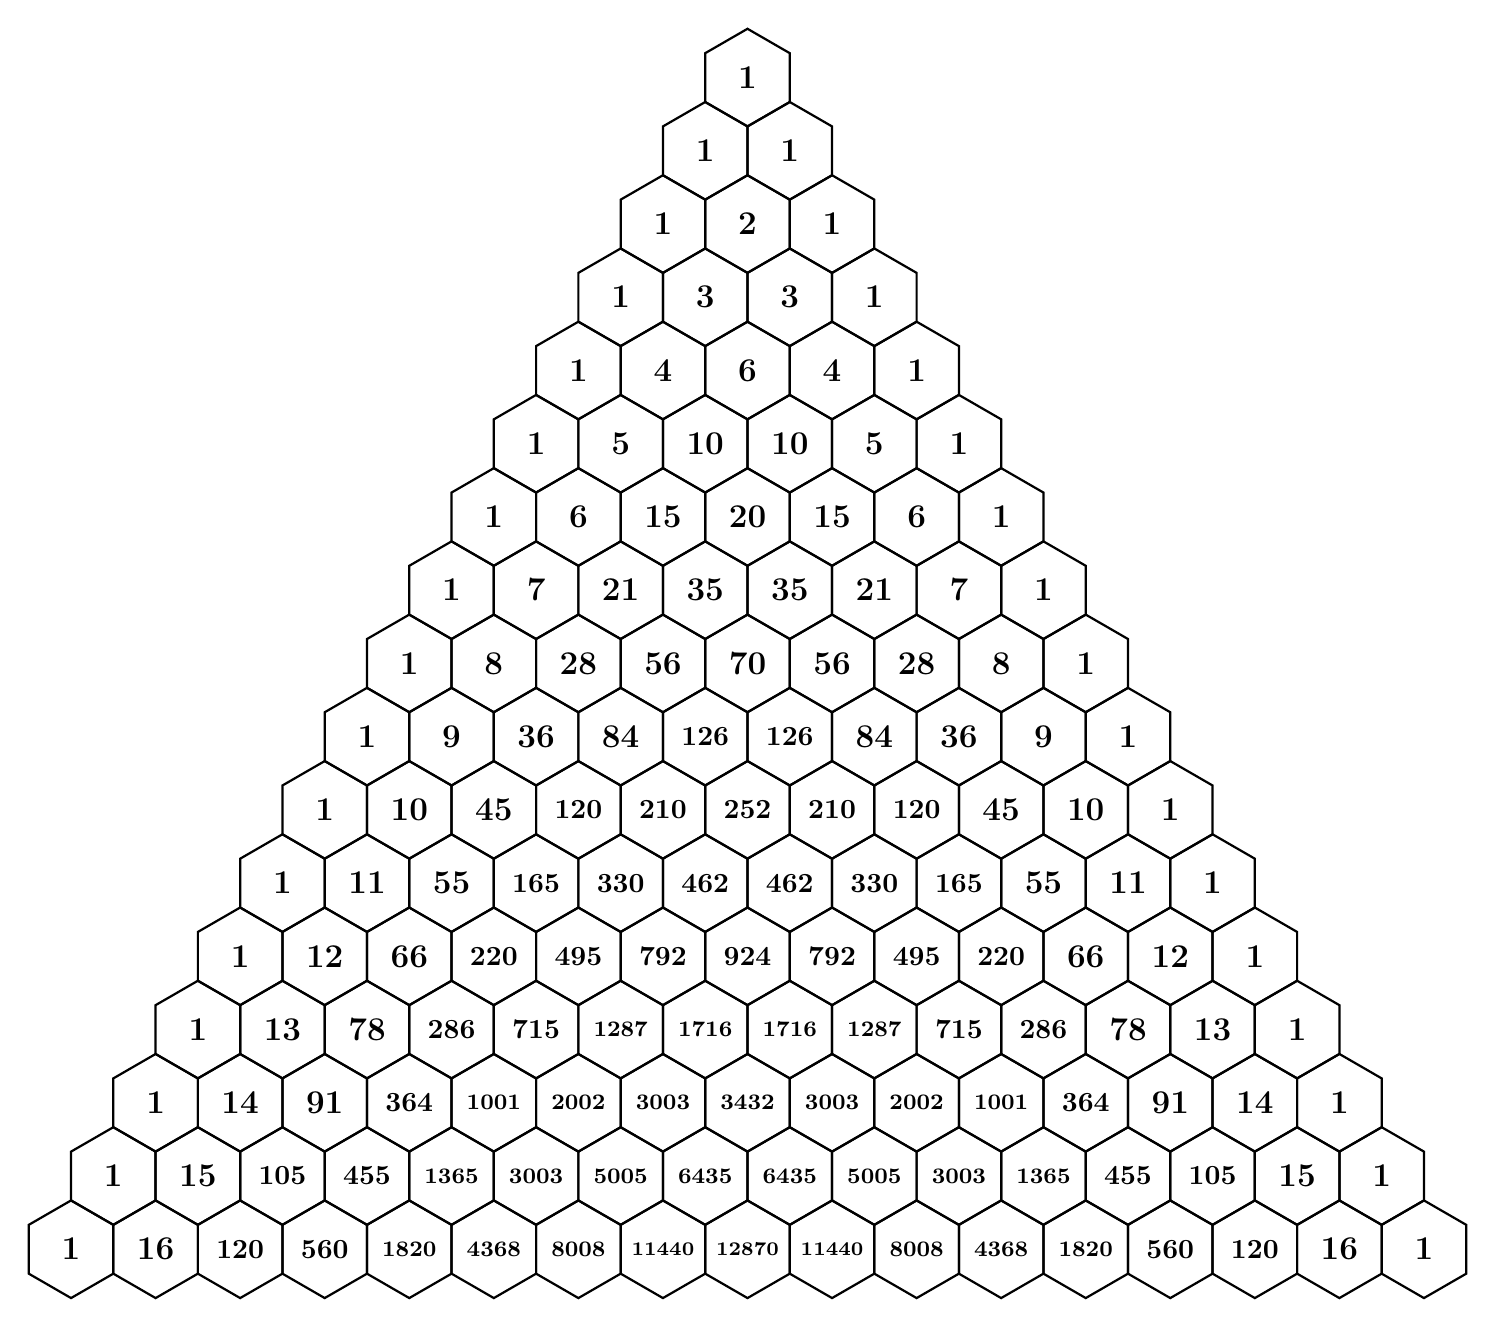
\begin{tikzpicture}
\def\r{.62}
\newcommand{\hexagon}[3]{
  \def\x{-cos{30}*\r*#1+cos{30}*#2*\r*2}
  \def\y{-\r*#1-sin{30}*\r*#1}
  \draw[thick] (\x,\y) +(90:\r) -- +(30:\r) -- +(-30:\r) -- +(-90:\r) -- +(-150:\r) -- +(150:\r) -- cycle;
  \draw (\x,\y) node{\bf #3};
}

  
% Pascal's triangle
%put row of 1's down left side:
  \foreach \row in {0,...,16} {
    \hexagon{\row}{0}{\large 1}
  }
%fill in the rest of the triangle:
  \foreach \row in {1,...,16} {
    \pgfmathsetmacro{\value}{1};
    \foreach \col in {1,...,\row} {
      % iterative formula : val = precval * (row-col+1)/col
      % (+ 0.5 to bypass rounding errors)
      \pgfmathtruncatemacro{\value}{\value*((\row-\col+1)/\col)+0.5};
      \global\let\value=\value
      \ifnum \value<100
	\hexagon{\row}{\col}{\large \value}
      \else \ifnum \value<1000
	\hexagon{\row}{\col}{\value}
      \else \ifnum \value<10000
	\hexagon{\row}{\col}{\footnotesize \value}
	\else
	\hexagon{\row}{\col}{\scriptsize \value}
	\fi
      \fi
      \fi
    }
  }
\end{tikzpicture}
\vfill
\end{center}



\end{document}


